\chapter{User Guided Synthesis of an \iic\ Driver}
\label{ch:worked_example}

In this appendix we will step through synthesis of the driver for a simple but real device. The device we are targeting is an \iic\ controller on a Samsung Exynos~5 system on ship. We assume the there is no operating system i.e.\ the driver runs on bare metal.

We start with the operating system specification. This gives us the interface that the driver is expected to provide. \iic\ is a bus protocol typically used to attach low speed devices to a processor. \iic\ transactions take place between a master device and a slave device. They are always initiated by the master, which may request a read or a write. Each device on an \iic\ bus has an address which is used by the master to identify the slave that it wants to communicate with. In this walkthrough, we will synthesise the driver code necessary to perform a write in master mode. 

\iic\ transactions occur in three phases:
\begin{enumerate}
    \item The transaction is initiated and the address of the slave that the master wants to communicate with is placed on the bus.
    \item The master sends some number $N$ of bytes.
    \item The master ends the transaction by sending a stop bit.
\end{enumerate}

\section{Driver template}

Our driver interface provides three functions, \code{send\_address()}, \code{send\_data()} and \code{send\_stop()}, one for each phase. In C code, the driver may be used like so:
\begin{figure}
\caption{Usage of the \iic driver}
\label{fig:iic_usage}
\begin{lstlisting}[frame=single]
send_address(0xAD);

//Call the below function as many times as you like:
send_data(dat0);
send_data(dat1);
send_data(dat2);

send_stop();
\end{lstlisting}
\end{figure}

Additionally, it provides a function called \code{configure()} that initialises the device so that it is ready to perform transactions.

We declare these required functions in the driver template (Listing~\ref{lst:drv_temp}):
\vspace*{5mm}
\lstinputlisting[style=tsl2, caption=Empty driver template, label=lst:drv_temp]{i2c/drv.tsl}
\vspace*{5mm}

Each function stub contains a magic block (\code{...;}) (Section~\ref{s:o:magic}). It is Termite's job to fill these function bodies in.

\section{Configuration}

\subsection{OS specification}

The OS specification, given in Listing~\ref{lst:os_spec}, describes when these driver functions may be called and what is expected of them. It is essentially a testbench that expresses requirements of the driver with assertions and goals.

The main TSL process (Section~\ref{s:o:execmodel}) is on line~\ref{l:os_pos}. The first thing it does is call \code{configure} (line~\ref{l:drv_configure}) in the driver. This is followed by a call to the procedure \code{configured} (line~\ref{l:os_configured}). It is the job of \code{configured} to check that \code{configure} in the driver did its job. It obtains various configuration parameters from the device specification (Section~\ref{a:sec:dev_spec}) and asserts that they are all initialised. 
        
Of course, it makes no sense for the OS to call functions in the device hardware, and this does not happen in reality. These are \emph{virtual functions} that are provided by the device specification to query its current state to enforce correct driver behaviour. 

\subsection{Device specification}
\label{a:sec:dev_spec}

The device specification, given in Listing~\ref{lst:dev_spec}, provides the mechanism for the driver to set the required configuration values as well as the means for the OS to query those values (through virtual functions). Configuration values are set through register writes such as \code{write8\_i2ccon} on line~\ref{l:dev_write8_i2ccon}. This code sets an internal register to the value written (line~\ref{l:dev_write8_i2ccon}) and optionally influences the state machine of an in-progress master transaction (Section~\ref{a:sec_master_write}). 

\code{ack\_enabled} on line~\ref{l:dev_ack_enabled} is an example virtual interface function. This is called by the OS specification in \code{configured} to check that the hardware sends acknowledge bits. To ensure that this return true as required, the driver must set bit 7 to one when writing to the \code{i2ccon} register.

When a configuration value is changed, the device calls the virtual OS callback function \code{config\_updated()} on line~\ref{l:dev_write8_i2ccon_cu}. This callback, defined on line~\ref{l:os_config_updated} of the OS specification, checks that the configuration parameters are still reasonable. This is needed because, for example, the register that is written to to initiate a master transaction also contains configuration information. This ensures that the driver always keeps correct data in these configuration fields when initiating transactions.

\subsection{Synthesising}
Ignoring the rest of the specification for now, we will attempt to synthesise the driver configuration function. We fire up Termite with \code{termite -i main.tsl -s}, it compiles the specifications and in less than a minute it has synthesised a strategy. A window, is created which allow the user to generate code in a user guided fashion. After navigating to the driver tab (Figure~\ref{fig:driver_tab}) we can begin code generation. If we place the cursor in the magic block in the configure function and then click on the \code{generate} button, a line of code will be automatically generated. Clicking the \code{generate} button again three more times completes the configuration function as indicated by the magic block being replaced by an empty block, as shown in Figure~\ref{fig:driver_tab_gen}. This generated code correctly initialises the device such that all the assertions in \code{configured} pass. This concludes generation of the \code{configure} function.

\begin{figure}
    \center
    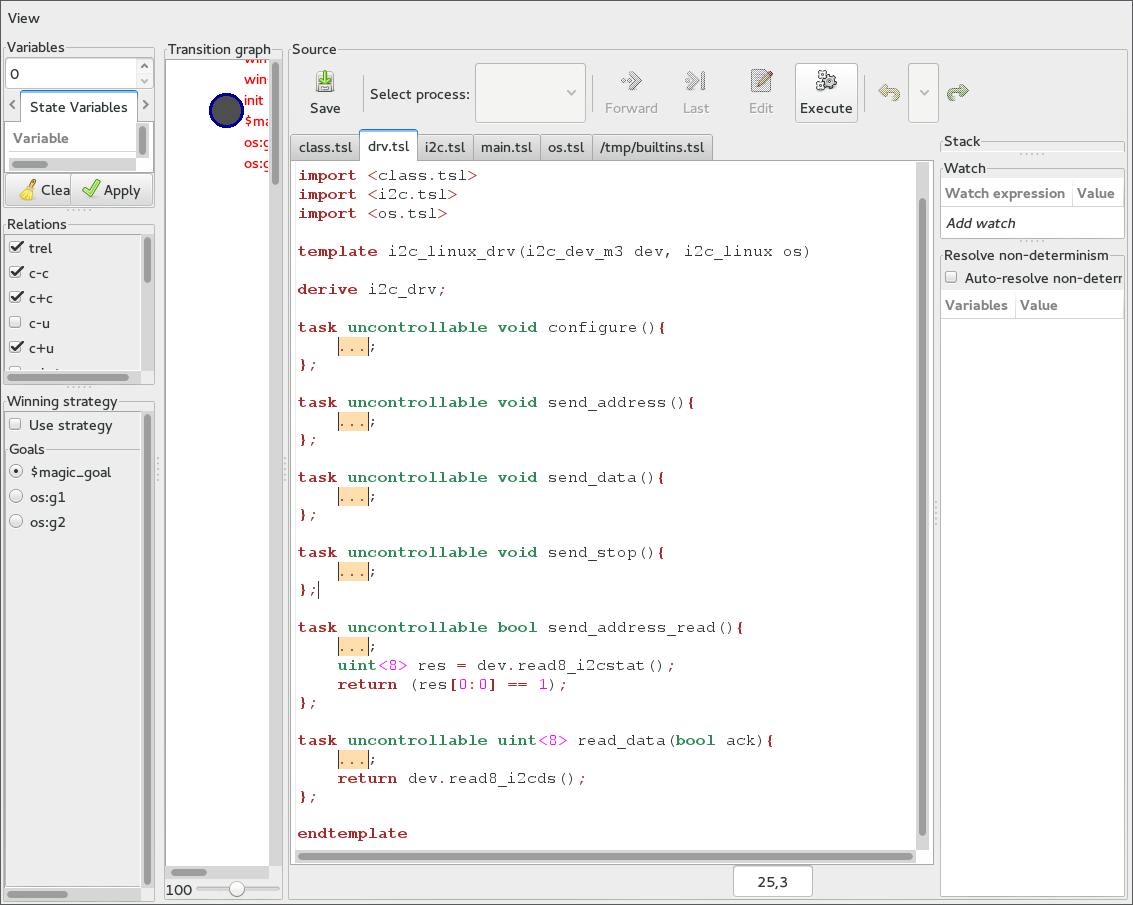
\includegraphics[width=\linewidth]{imgs/screenshot_1.png}
    \caption{Termite driver source code tab}
    \label{fig:driver_tab}
\end{figure}

\begin{figure}
    \center
    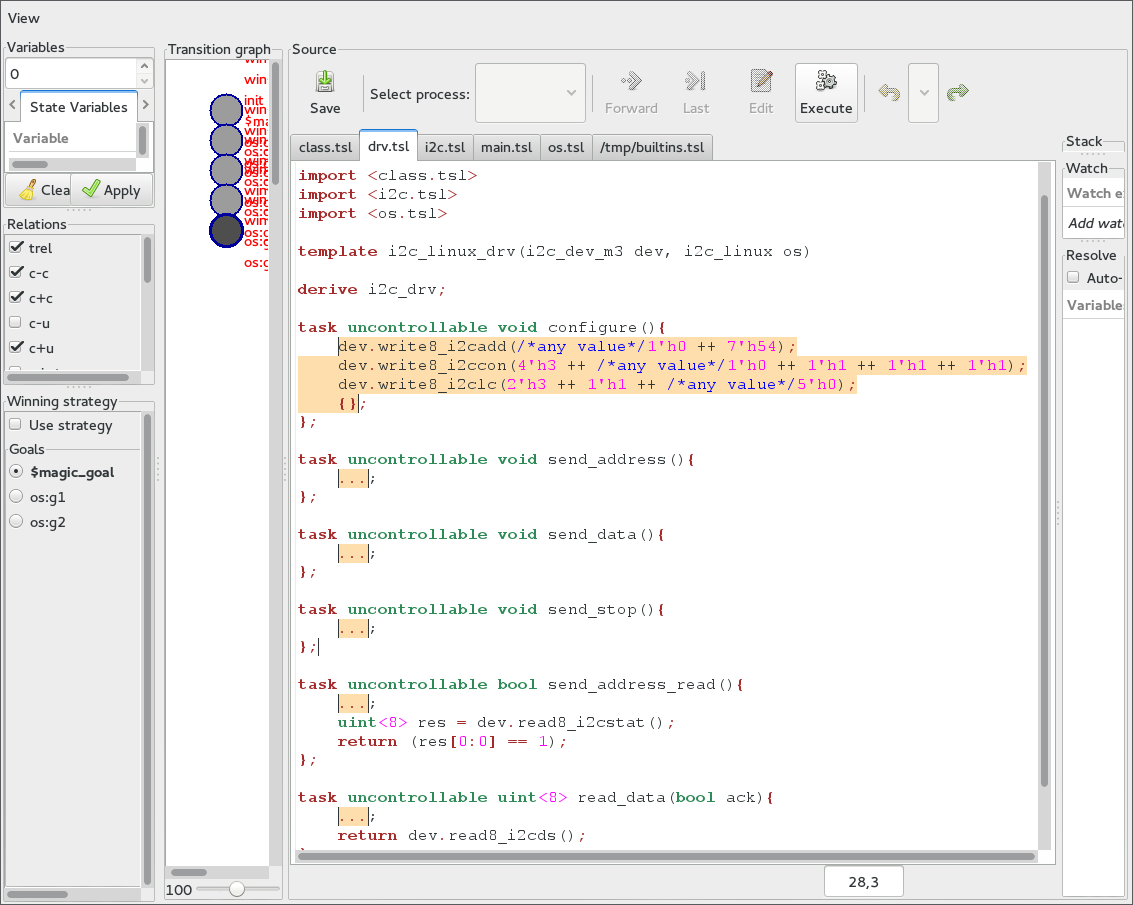
\includegraphics[width=\linewidth]{imgs/screenshot_2.png}
    \caption{Termite driver source code tab after code generation}
    \label{fig:driver_tab_gen}
\end{figure}

\section{Master write}
\label{a:sec_master_write}

\subsection{OS specification}
We continue from where we left off in the \code{pos} process in the OS specification. We first set a flag to signal that initialisation was successful and then we enter a forever loop (Section~\ref{sec:loops}). On each iteration, the loop non-deterministically chooses between performing a master read or a master write transaction. We do not cover synthesis of the master read transaction. Assuming execution of the process enters the \code{master\_write} function we end up at line~\ref{l:os_master_write}.

This function models the behaviour we expect of the \code{send\_address}, \code{send\_data} and \code{send\_stop} sequence of driver functions. It uses a state variable \code{master\_state} to keep track of the current state of the master transmission. 

Note the two \emph{virtual callbacks} (similar to virtual functions) \code{address\_written} and \code{data\_sent} defined on lines~\ref{l:os_address_written} and~\ref{l:os_data_sent} respectively. They are invoked by the device state machine when the address writing and data sending phases complete. 

\subsection{Device specification}
As with configuration, the device specification must provide the mechanism for the driver to perform the master write transaction. Again this is performed through register writes such as \code{write8\_i2cstat} on line~\ref{l:dev_write8_i2cstat}. Observe that if bit 5 is set and there is currently no master transaction in progress, in addition to writing to the internal register, the write initiates a transaction by setting the enumeration \code{master\_transmit\_st} to \code{transmitting\_adddress\_t}. 

Process \code{pmaster} (line~\ref{l:dev_pmaster}) is the main device process responsible for performing the master transaction. \code{pmaster} is non-deterministically scheduled to run when events happen in the master state machine. When 
$$
\code{master\_transmit\_st} == \code{transmitting\_address\_t} 
$$
(as set by a previous write to \code{i2cstat}) on line~\ref{l:dev_pmaster_ta} it signals to the operating system that the address was written using the \code{address\_written} callback on line~\ref{l:dev_pmaster_aw}, which triggers the operating system to update its internal state.

Process \code{pmaster} handles data and stop bit transmission in the same way.

\subsection{Synthesising}

\begin{figure}
    \center
    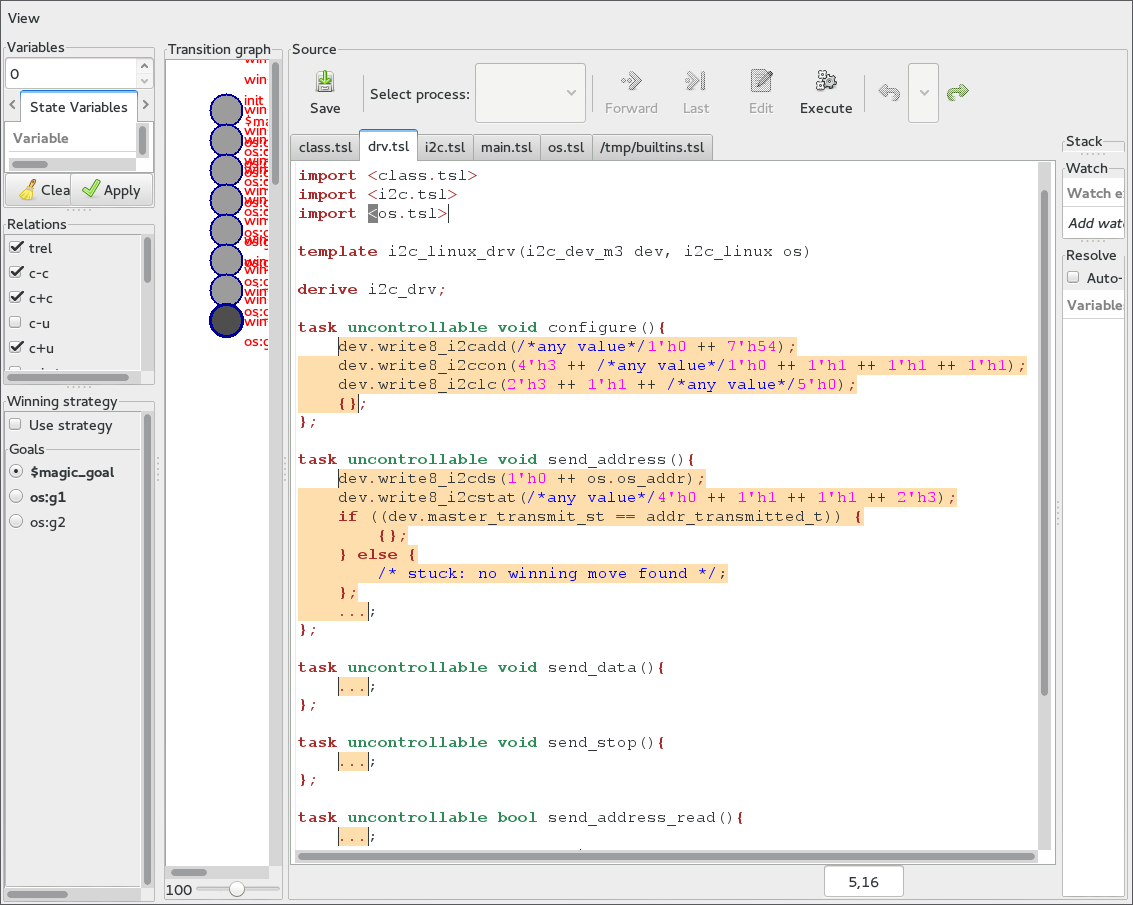
\includegraphics[width=\linewidth]{imgs/screenshot_3.png}
    \caption{Termite driver source code tab. Sending address.}
    \label{fig:driver_tab_addr}
\end{figure}

We proceed to generate code as we did for configuration. Code generation for \code{send\_address()} is shown in Figure~\ref{fig:driver_tab_addr}. The first two lines are generated automatically as before. However, on the third line, Termite gets stuck. It generates an if condition that says that if the device specification internal state variable \code{master\_transmit\_st} is equal to \code{addr\_transmitted\_t} then we can return from this function, otherwise, Termite is stuck. There are two problems with this code: the device internal variable is not accessible to the driver, and, one branch of the if statement is a dead end. 

This is actually Termite's rather cryptic way of saying that the correct action is to wait until $\code{dev.master\_transmit\_st} == \code{addr\_transmitted\_t}$. This corresponds to waiting until the address is transmitted, which is what you would expect. The driver developer can verify this by replacing the entire if condition with 

$$\code{wait(dev.master\_transmit\_st} == \code{addr\_transmitted\_t})$$.

This is a manifestation of the white box assumption that Termite makes. It assumes that the driver can access all of the system's state variables. To remedy this, manual intervention is needed. Consultation of the device manual tells us that after the address is sent the device sets bit 4 of \code{i2ccon} to one. So, we manually write code to loop while this bit is zero (line~\ref{l:drv_manual_loop}). We then re-run Termite with the amended driver and Termite checks that the manually written code is correct. Synthesis with the manually written code succeeds and, again, Termite creates the window shown in Figure~\ref{fig:driver_tab_addr_man}, verifying that the code is correct. So, while we were forced to write code manually, Termite was able to verify that is was correct.

\begin{figure}
    \center
    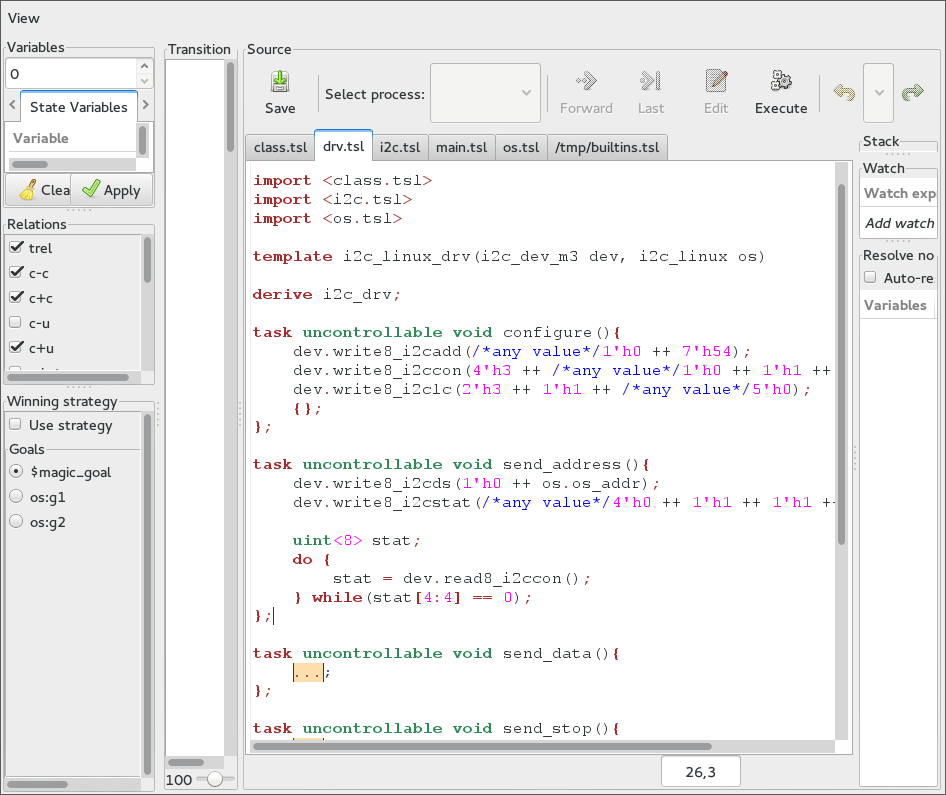
\includegraphics[width=\linewidth]{imgs/screenshot_4.png}
    \caption{Termite driver source code tab. Sending address manual code.}
    \label{fig:driver_tab_addr_man}
\end{figure}

We proceed in exactly the same way for the remaining functions \code{send\_data()} and \code{send\_stop()}. Each function requires us to manually work around the white box assumption as we did for \code{send\_address()}. The final driver is shown in Listing~\ref{lst:synth}.

\section{Specifications}

In this section we give all specifications in full. In addition to the specifications already discussed, we also give the class specification (Listing~\ref{lst:class_spec}) and the main file (Listing~\ref{lst:main}). The class specification is much like C header and it declares datatypes and the externally visible interface to the other specifications. The main file creates an instance of each specification and ties them together.

\vspace*{5mm}
\lstinputlisting[style=tsl2, caption=OS specification, label=lst:os_spec]{i2c/os.tsl}
\vspace*{5mm}
\lstinputlisting[style=tsl2, caption=Device specification, label=lst:dev_spec]{i2c/i2c.tsl}
\vspace*{5mm}
\lstinputlisting[style=tsl2, caption=Class specification, label=lst:class_spec]{i2c/class.tsl}
\vspace*{5mm}
\lstinputlisting[style=tsl2, caption=Main file, label=lst:main]{i2c/main.tsl}
\vspace*{5mm}
\lstinputlisting[style=tsl2, caption=Synthesised driver, label=lst:synth]{i2c/drv.tsl.synthesized}

